\documentclass[tikz,border=2pt]{standalone}

\usepackage[T1]{fontenc}
\usepackage[utf8]{inputenc}
\usepackage{times}
\usepackage{xcolor}
\definecolor{paperMauve}{HTML}{8839EF}
\definecolor{paperRed}{HTML}{D20F39}
\definecolor{paperTeal}{HTML}{179299}
\definecolor{paperBlue}{HTML}{1E66F5}
\definecolor{paperText}{HTML}{4C4F69}
\definecolor{paperSubtextZero}{HTML}{6C6F85}
\definecolor{paperOverlayOne}{HTML}{8C8FA1}
\definecolor{paperSurfaceZero}{HTML}{CCD0DA}


\begin{document}

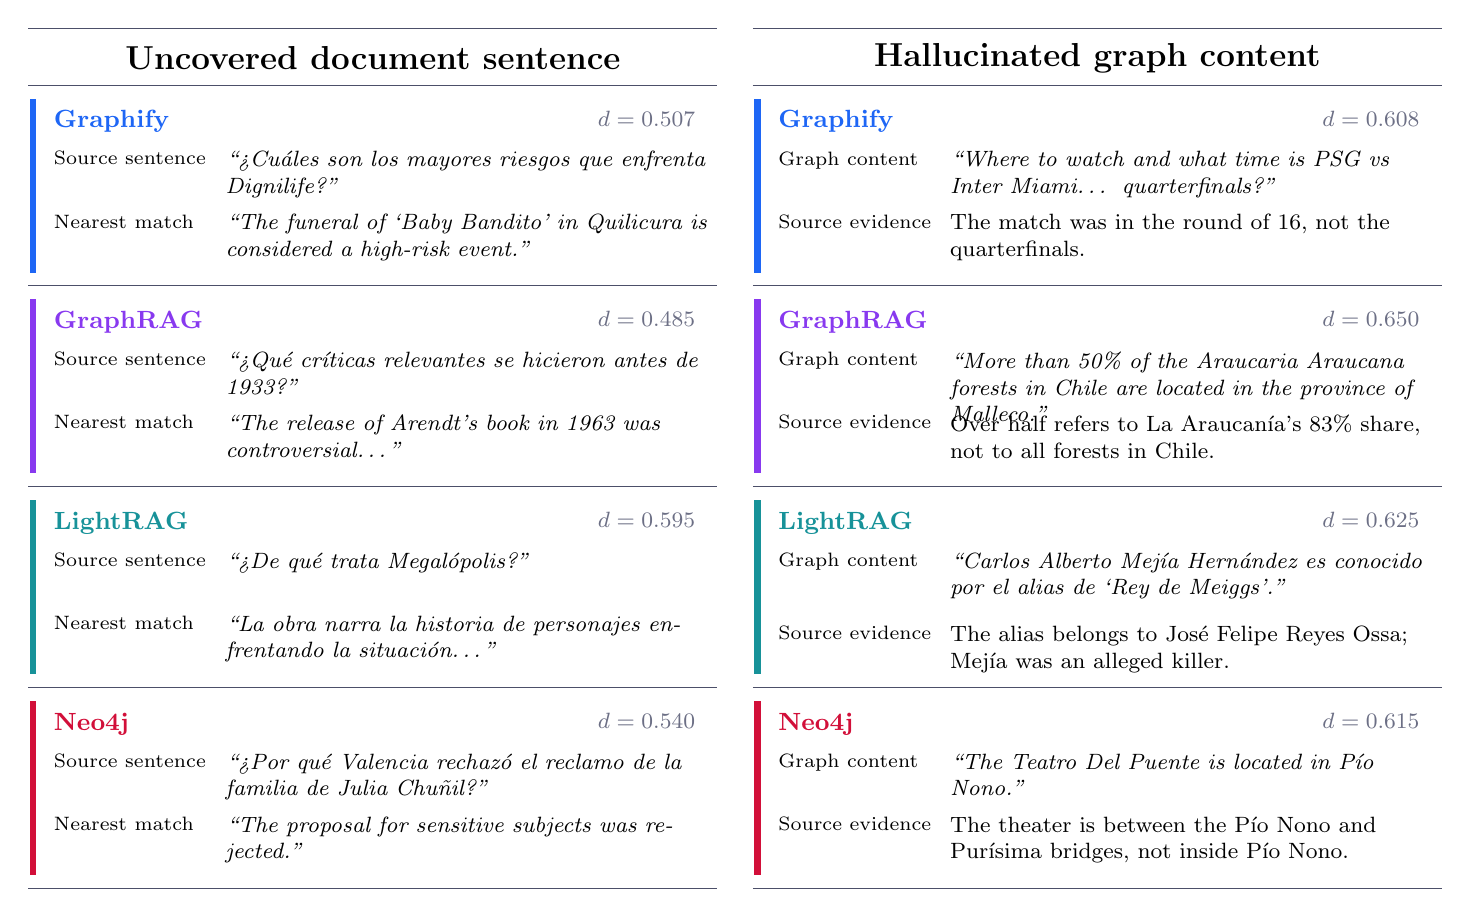
\begin{tikzpicture}[
    font=\rmfamily,
    coltitle/.style={font=\rmfamily\bfseries\large, anchor=center,
      align=center, text width=8.1cm},
    program/.style={font=\rmfamily\bfseries\small, anchor=north west},
    distlabel/.style={font=\rmfamily\footnotesize, anchor=north east,
      text=paperSubtextZero},
    field/.style={font=\rmfamily\scriptsize, anchor=north west},
    body/.style={font=\rmfamily\footnotesize, align=left,
      text width=6.15cm, anchor=north west},
    excerpt/.style={font=\rmfamily\itshape\footnotesize, align=left,
      text width=6.15cm, anchor=north west},
    rightbody/.style={font=\rmfamily\footnotesize, align=left,
      text width=6.15cm, anchor=north west},
    rightexcerpt/.style={font=\rmfamily\itshape\footnotesize, align=left,
      text width=6.15cm, anchor=north west},
    rule/.style={draw=paperText, line width=0.55pt},
    lightRule/.style={draw=paperText, line width=0.35pt}
  ]

  \def\colW{8.75}
  \def\rightX{9.20}
  \def\labelX{0.20}
  \def\textX{2.38}
  \def\rightTextX{2.38}
  \def\topY{0}
  \def\titleY{-0.38}
  \def\headerRuleY{-0.72}
  \def\rowOneY{-0.72}
  \def\rowTwoY{-3.27}
  \def\rowThreeY{-5.82}
  \def\rowFourY{-8.37}
  \def\bottomY{-10.92}

  \colorlet{graphifyColor}{paperBlue}
  \colorlet{graphragColor}{paperMauve}
  \colorlet{lightragColor}{paperTeal}
  \colorlet{neoColor}{paperRed}

  \foreach \x/\title in {0/Uncovered document sentence,
      \rightX/Hallucinated graph content} {
    \draw[rule] (\x,\topY) -- ++(\colW,0);
    \draw[lightRule] (\x,\headerRuleY) -- ++(\colW,0);
    \draw[lightRule] (\x,\rowOneY) -- ++(\colW,0);
    \draw[lightRule] (\x,\rowTwoY) -- ++(\colW,0);
    \draw[lightRule] (\x,\rowThreeY) -- ++(\colW,0);
    \draw[lightRule] (\x,\rowFourY) -- ++(\colW,0);
    \draw[rule] (\x,\bottomY) -- ++(\colW,0);
    \node[coltitle] at ({\x + 0.5*\colW},\titleY) {\title};
  }

  \foreach \x in {0,\rightX} {
    \fill[graphifyColor] ({\x+0.02},{\rowOneY-0.17})
      rectangle ({\x+0.10},{\rowTwoY+0.17});
    \fill[graphragColor] ({\x+0.02},{\rowTwoY-0.17})
      rectangle ({\x+0.10},{\rowThreeY+0.17});
    \fill[lightragColor] ({\x+0.02},{\rowThreeY-0.17})
      rectangle ({\x+0.10},{\rowFourY+0.17});
    \fill[neoColor] ({\x+0.02},{\rowFourY-0.17})
      rectangle ({\x+0.10},{\bottomY+0.17});
  }

  \node[program, text=graphifyColor] at (\labelX,{\rowOneY-0.20})
    {Graphify};
  \node[distlabel] at ({\colW-0.16},{\rowOneY-0.20}) {$d=0.507$};
  \node[field] at (\labelX,{\rowOneY-0.72}) {Source sentence};
  \node[excerpt] at (\textX,{\rowOneY-0.72})
    {``¿Cuáles son los mayores riesgos que enfrenta Dignilife?''};
  \node[field] at (\labelX,{\rowOneY-1.52}) {Nearest match};
  \node[excerpt] at (\textX,{\rowOneY-1.52})
    {``The funeral of `Baby Bandito' in Quilicura is considered a
    high-risk event.''};

  \node[program, text=graphifyColor]
    at ({\rightX+\labelX},{\rowOneY-0.20}) {Graphify};
  \node[distlabel]
    at ({\rightX+\colW-0.16},{\rowOneY-0.20}) {$d=0.608$};
  \node[field] at ({\rightX+\labelX},{\rowOneY-0.72}) {Graph content};
  \node[rightexcerpt] at ({\rightX+\rightTextX},{\rowOneY-0.72})
    {``Where to watch and what time is PSG vs Inter Miami\ldots{}
    quarterfinals?''};
  \node[field] at ({\rightX+\labelX},{\rowOneY-1.52}) {Source evidence};
  \node[rightbody] at ({\rightX+\rightTextX},{\rowOneY-1.52})
    {The match was in the round of 16, not the quarterfinals.};

  \node[program, text=graphragColor] at (\labelX,{\rowTwoY-0.20})
    {GraphRAG};
  \node[distlabel] at ({\colW-0.16},{\rowTwoY-0.20}) {$d=0.485$};
  \node[field] at (\labelX,{\rowTwoY-0.72}) {Source sentence};
  \node[excerpt] at (\textX,{\rowTwoY-0.72})
    {``¿Qué críticas relevantes se hicieron antes de 1933?''};
  \node[field] at (\labelX,{\rowTwoY-1.52}) {Nearest match};
  \node[excerpt] at (\textX,{\rowTwoY-1.52})
    {``The release of Arendt's book in 1963 was controversial\ldots''};

  \node[program, text=graphragColor]
    at ({\rightX+\labelX},{\rowTwoY-0.20}) {GraphRAG};
  \node[distlabel]
    at ({\rightX+\colW-0.16},{\rowTwoY-0.20}) {$d=0.650$};
  \node[field] at ({\rightX+\labelX},{\rowTwoY-0.72}) {Graph content};
  \node[rightexcerpt] at ({\rightX+\rightTextX},{\rowTwoY-0.72})
    {``More than 50\% of the Araucaria Araucana forests in Chile are
    located in the province of Malleco.''};
  \node[field] at ({\rightX+\labelX},{\rowTwoY-1.52}) {Source evidence};
  \node[rightbody] at ({\rightX+\rightTextX},{\rowTwoY-1.52})
    {Over half refers to La Araucanía's 83\% share, not to all forests
    in Chile.};

  \node[program, text=lightragColor] at (\labelX,{\rowThreeY-0.20})
    {LightRAG};
  \node[distlabel] at ({\colW-0.16},{\rowThreeY-0.20}) {$d=0.595$};
  \node[field] at (\labelX,{\rowThreeY-0.72}) {Source sentence};
  \node[excerpt] at (\textX,{\rowThreeY-0.72})
    {``¿De qué trata \textit{Megalópolis}?''};
  \node[field] at (\labelX,{\rowThreeY-1.52}) {Nearest match};
  \node[excerpt] at (\textX,{\rowThreeY-1.52})
    {``La obra narra la historia de personajes enfrentando la
    situación\ldots''};

  \node[program, text=lightragColor]
    at ({\rightX+\labelX},{\rowThreeY-0.20}) {LightRAG};
  \node[distlabel]
    at ({\rightX+\colW-0.16},{\rowThreeY-0.20}) {$d=0.625$};
  \node[field] at ({\rightX+\labelX},{\rowThreeY-0.72}) {Graph content};
  \node[rightexcerpt] at ({\rightX+\rightTextX},{\rowThreeY-0.72})
    {``Carlos Alberto Mejía Hernández es conocido por el alias de
    `Rey de Meiggs'.''};
  \node[field] at ({\rightX+\labelX},{\rowThreeY-1.65}) {Source evidence};
  \node[rightbody] at ({\rightX+\rightTextX},{\rowThreeY-1.65})
    {The alias belongs to José Felipe Reyes Ossa; Mejía was an alleged
    killer.};

  \node[program, text=neoColor] at (\labelX,{\rowFourY-0.20}) {Neo4j};
  \node[distlabel] at ({\colW-0.16},{\rowFourY-0.20}) {$d=0.540$};
  \node[field] at (\labelX,{\rowFourY-0.72}) {Source sentence};
  \node[excerpt] at (\textX,{\rowFourY-0.72})
    {``¿Por qué Valencia rechazó el reclamo de la familia de Julia
    Chuñil?''};
  \node[field] at (\labelX,{\rowFourY-1.52}) {Nearest match};
  \node[excerpt] at (\textX,{\rowFourY-1.52})
    {``The proposal for sensitive subjects was rejected.''};

  \node[program, text=neoColor]
    at ({\rightX+\labelX},{\rowFourY-0.20}) {Neo4j};
  \node[distlabel]
    at ({\rightX+\colW-0.16},{\rowFourY-0.20}) {$d=0.615$};
  \node[field] at ({\rightX+\labelX},{\rowFourY-0.72}) {Graph content};
  \node[rightexcerpt] at ({\rightX+\rightTextX},{\rowFourY-0.72})
    {``The Teatro Del Puente is located in Pío Nono.''};
  \node[field] at ({\rightX+\labelX},{\rowFourY-1.52}) {Source evidence};
  \node[rightbody] at ({\rightX+\rightTextX},{\rowFourY-1.52})
    {The theater is between the Pío Nono and Purísima bridges, not
    inside Pío Nono.};

\end{tikzpicture}

\end{document}
